Das Backend soll wie in Kapitel 2.3 beschrieben die Datenquelle f�r die
verschiedenen Clients sein. Umgesetzt werden soll dies �ber einen RESTful
Service. Es wird das Framework "`Spring"' eingesetzt. Dies erlaubt eine einfache
Erstellung von Web-Services und unterst�tzt den Programmierer mit Werkzeugen wie
Hibernate, die die Verwaltung der Datenbank stark vereinfacht und �nderungen an
der Modellierung direkt in der Datenbank umsetzt.
\subsection{Anforderungen}
Das Backend soll den Clients die Daten wie oben genannt �ber einen
RESTful-Service zur Verf�gung stellen. Dies vereinfacht den Zugriff auf die
Ressourcen und ist leicht in bestehende Infrastrukturen einzubinden. Das Backend
soll nach M�glichkeit �ber \ac{https} zur Verf�gung stellen, damit �bertragene
Daten auf dem Weg gesichert sind. Eine Authentifizierung auf Zugriffsebene ist
optional, da der Service in einem geschlossenen Netz betrieben werden soll. Das
Backend soll zudem Authentifizierungsanfragen auf Anwendungsebene bearbeiten. 
\subsection{Implementierung}
	Das Backend wird mit dem quelloffenen Framework Spring umgesetzt. Spring bietet
	wie in Kapitel
	\subsubsection{Datenbank}
	
	 \begin{figure}[H]
		\begin{minipage}{\linewidth}
		 	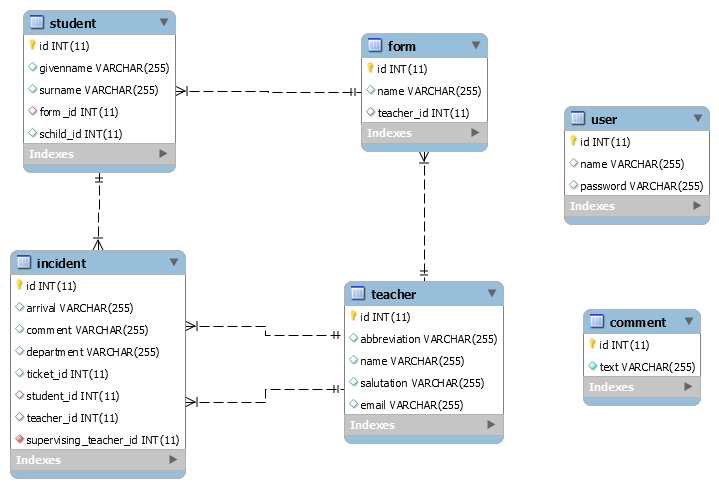
\includegraphics[width=0.9\linewidth]{grafx/ER_Model}
 			\caption[ER-Modell der Datenbank]{ER-Modell der Datenbank}
  			\label{fig:er_model}
		\end{minipage}
	\end{figure}

\subsection{Tests }


	\subsubsection{In Memory DB ?}


\subsection{Generischer Controller ??}
 